%%%%%%%%%%%%%%%%%%%%
% Copyright and authorship: Fernando Oleo Blanco.
%
% Thanks to all the people that helped me get to where I am.
% Free use, just acknowledge the authors.
%%%%%%%%%%%%%%%%%%%%

\documentclass[12pt, a4paper]{book} % General document definition. In order to have the text completely centered, do not use the twoside option; however, twoside is recommended for printing.

% For general information and help, refer to https://www.overleaf.com/learn

%% PACKAGES

\usepackage[utf8]{inputenc} % Set the utf8 input encoding
\usepackage[spanish]{babel} % Select your prefered language. Example: \usepackage[activeacute,spanish]{babel}
\usepackage{amsmath, amsfonts, amssymb} % Mathematical notation
\usepackage{fancyhdr} % Header and footer customization
\setlength{\headheight}{16pt} % Increase headheight to avoid fancyhdr warnings
\usepackage{titlesec} % Section printing customization
\usepackage{graphicx} % Graphics import and tools
\usepackage{color} % To use colors in the document
\usepackage{geometry} % To modify the geometry of pages (margins and other lengths)
\usepackage{hyperref} % "Advance" and easier referencing
\usepackage{listings} % To add and format code. See https://www.overleaf.com/learn/latex/Using_listings_to_format_source_code for more information
\usepackage{csquotes} % Recommended for biblatex with babel/polyglossia
\usepackage{xcolor} % Adds more colors to the available list
\usepackage[final]{pdfpages} % Includes pdfs directly, not as images
\usepackage{lipsum} % Dummy text to test the design
\usepackage[backend=biber,
			style=numeric,
			citestyle=numeric,
			sorting=none]{biblatex}
		% Citation configuration. We use biblatex, which is more
        % complex, but as customizable as it gets.
        % Please, modify this to your liking.
        % IMPORTANT: this requires biber to be installed and run every time
        % you change the .bib file! To make it easier, if you are using TeXStudio, do the following:
        % 1. Go to options. 2. Select the Build menu. 3 In standard bibliography, change bibtex to biber. 4. Profit
        % These changes will allow the editor to detect any changes and "recompile" the files if needed.
        % For other editors see: https://tex.stackexchange.com/questions/154751/biblatex-with-biber-configuring-my-editor-to-avoid-undefined-citations
       	% See link for a quick introduction: https://tex.stackexchange.com/questions/26516/how-to-use-biber/34136
        % If you are having issues with the bibliography, please, search for how to install and run biber!
        
% Specialised packages
\usepackage{tikz} % To create diagrams and figures
\usetikzlibrary{shapes, arrows, positioning, calc} % Tikz libraries for shapes and arrows
\usepackage{tikz-qtree} % To create trees with Tikz
\usepackage{pgfplotstable} % To create tables with Tikz
\usepackage{pgfplots} % Create native LaTeX looking plots (other backends are available)
\pgfplotsset{compat=1.18} % Set pgfplots compatibility version
\usepackage{todonotes} % Graphically create TODO entries
\usepackage{pgfplots} % Create native LaTeX looking plots (other backends are available)
\usepackage{todonotes} % Graphically create TODO entries
\usepackage{siunitx} % Write Units in accordance with the SI organization
\usepackage{eurosym} % Official Euro symbol
\usepackage{caption} % To customize captions
\usepackage{subcaption} % To create subcaptions for figures and tables
\usepackage{float} % To control the placement of figures and tables
\usepackage{tabularx}
\usepackage{colortbl}
\usepackage{pifont}
\usepackage{booktabs} % To create better tables
\usepackage{longtable} % To create tables that span multiple pages
\usepackage{multirow} % To create multirow cells in tables
\usepackage{enumitem} % To customize lists
\usepackage{setspace} % To set the line spacing
\usepackage{microtype} % To improve the typography of the document
\usepackage{array}
\usepackage{tikz-cd} % To create commutative diagrams
\usepackage{pgfplots} % To create plots with Tikz
\usepackage{pgfplotstable} % To create tables with Tikz
\usetikzlibrary{positioning}
\usetikzlibrary{shapes, arrows.meta, positioning}

% Entorno personalizado para los pasos conectados
\newcommand{\modelstep}[2]{
  \noindent
  \begin{tikzpicture}[baseline=(text.base)]
    \node[anchor=base west, inner sep=0pt] (text) {#2};
    \node[left=1em of text.base west, minimum width=1pt] (dot) {};
    \draw[very thick, -{Latex[length=2mm]}, gray]
      ($(dot)+(0,-0.6em)$) -- (dot);
  \end{tikzpicture}
}

%% PACKAGE CONFIGURATION

% Bibliography resource
\addbibresource{main.bib}

% Header and footer customization
\fancyhf{}
\fancyhead[LE]{\slshape \leftmark}
\fancyhead[RO]{\slshape \nouppercase \rightmark}
\fancyfoot[LE, RO]{\thepage}
% IMPORTANT! If your chapter/section names are too long to nicely fit on the header, use the shortened variant:
% \chapter[short tile]{actual long title} or \section[short title]{actual long title, title}

%% CUSTOM COMMANDS

% Add abstract environment to book style
\newenvironment{abstract}%
{\cleardoublepage \null \vfill \begin{center}%
		\bfseries \abstractname \end{center}}%
{\vfill\null}

%% DOCUMENT

\begin{document}
	
	\frontmatter % First few pages
	\pagestyle{empty} % We suppress the "fancy" hearders in the front matter
	
	% This creates a basic title page based on the one proposed by Comillas University.
	\begin{titlepage}
		\begin{figure}
			\centering
			
\includegraphics[width=0.3\linewidth]{LogoUniversidadBN}
		\end{figure}
		\centering
		\Large Grado en Ingeniería en Tecnologías de Telecomunicación \\ % Modify accordingly
		\vspace*{2.5em} % This just adds some vertical spacing
		\centering
		Trabajo fin de grado \\ % Modify accordingly
		\vspace*{1em}
		IA GENERATIVA PARA LA PREDICCIÓN Y GESTIÓN DE LA DEMANDA ENERGÉTICA % Write here the title of your study
		\\ \large
		\vspace*{3em}
		Autor \\ Álvaro González Tabernero \\ % Your name
		\vspace*{1em}
		Directores \\ Francisco Martín Martínez \\ Jaime Boal Martín-Larrauri % Supervisor(s) name(s) 
		%{\vfill \vspace*{3em}{Author's signature:\hrulefill \hfill} \hfill \\ \vspace*{4em}Supervisors' signatures:\hrulefill \hfill} % Uncoment this line if you would like to add a signature space
		\vfill
		Madrid \\
		Junio 2025 % Modify accordingly
	\end{titlepage}
	% Write your abstract
	\begin{abstract}
		Abstract content
	\end{abstract}

	\newpage

	% Coment this block if you don't want a general information page
	% Thanks and other information page
	{\centering Agradecimientos\\}
	\vfill % Fill the page with whitespace (this is just for aesthetical reasons)

	\cleardoublepage % New page starts on the right hand side
	
	\tableofcontents % Create the index
	\listoffigures % Create index of figures
	\listoftables % Create index of tables
	%\lstlistoflistings % Create index for code sections
	
	\cleardoublepage % Open on right hand page (odd numbered)
	
	\mainmatter 
	% Activate customized headers
	\pagestyle{fancy}
	\chapter{Introducción}
El acceso seguro y fiable a la electricidad es clave para el desarrollo económico y social de
cualquier sociedad. Con el aumento de la demanda energética, se está acelerando la adopción
de energías renovables para combatir el cambio climático y reducir la dependencia de
combustibles fósiles\\%cite{quest2022indicator}.\\

La descarbonización del sistema energético y la mejora de la eficiencia en el uso de los
recursos presentan retos en la optimización de la producción, la gestión de la demanda y la
estabilidad de la red. Las infraestructuras deben adaptarse para integrar de forma eficiente
las energías renovables, sin aumentar los costes ni comprometer la calidad del suministro\\%\cite{khenissi2021pso}.\\

El consumo energético en los hogares ha evolucionado significativamente en los últimos años,
con un aumento en el uso de dispositivos electrónicos, electrodomésticos con mayor capacidad 
computacional y el auge del vehículo eléctrico (EV). Éste se ha convertido en una parte 
esencial de la transición hacia una movilidad más sostenible, pero su integración plantea 
desafíos significativos en términos de gestión de la demanda y estabilidad de la red 
eléctrica.\\

Los EV y vehículos híbridos enchufables (PHEV, por sus siglas en inglés) lejos están de ser 
tecnología del futuro, son el presente. Los EV y vehículos electrificados han cambiado por completo
el paradigma energético doméstico, convirtiéndose en una parte integral de la vida cotidiana%\cite{truong2021occupancy}.
La adopción de estos vehículos ha crecido exponencialmente en los últimos años, impulsada por
la necesidad de reducir las emisiones de gases de efecto invernadero y la dependencia de los
combustibles fósiles. En España, el número de vehículos eléctricos ha aumentado considerablemente,
con una creciente infraestructura de carga y un interés cada vez mayor por parte de los
consumidores.\\  

La carga de estos vehículos eléctricos puede generar picos de demanda que, de no ser
gestionados adecuadamente, podrían llegar a comprometer la fiabilidad de la red y aumentar 
significativamente los costes operativos~\cite{yao2005energy}, repercutiendo finalmente en los consumidores.
La \hyperref[fig:ev_interest]{\figurename~\ref*{fig:ev_interest}} muestra la evolución del 
interés por los EV en España durante los útlimos diez años\\

\begin{figure}[ht]
    \centering
    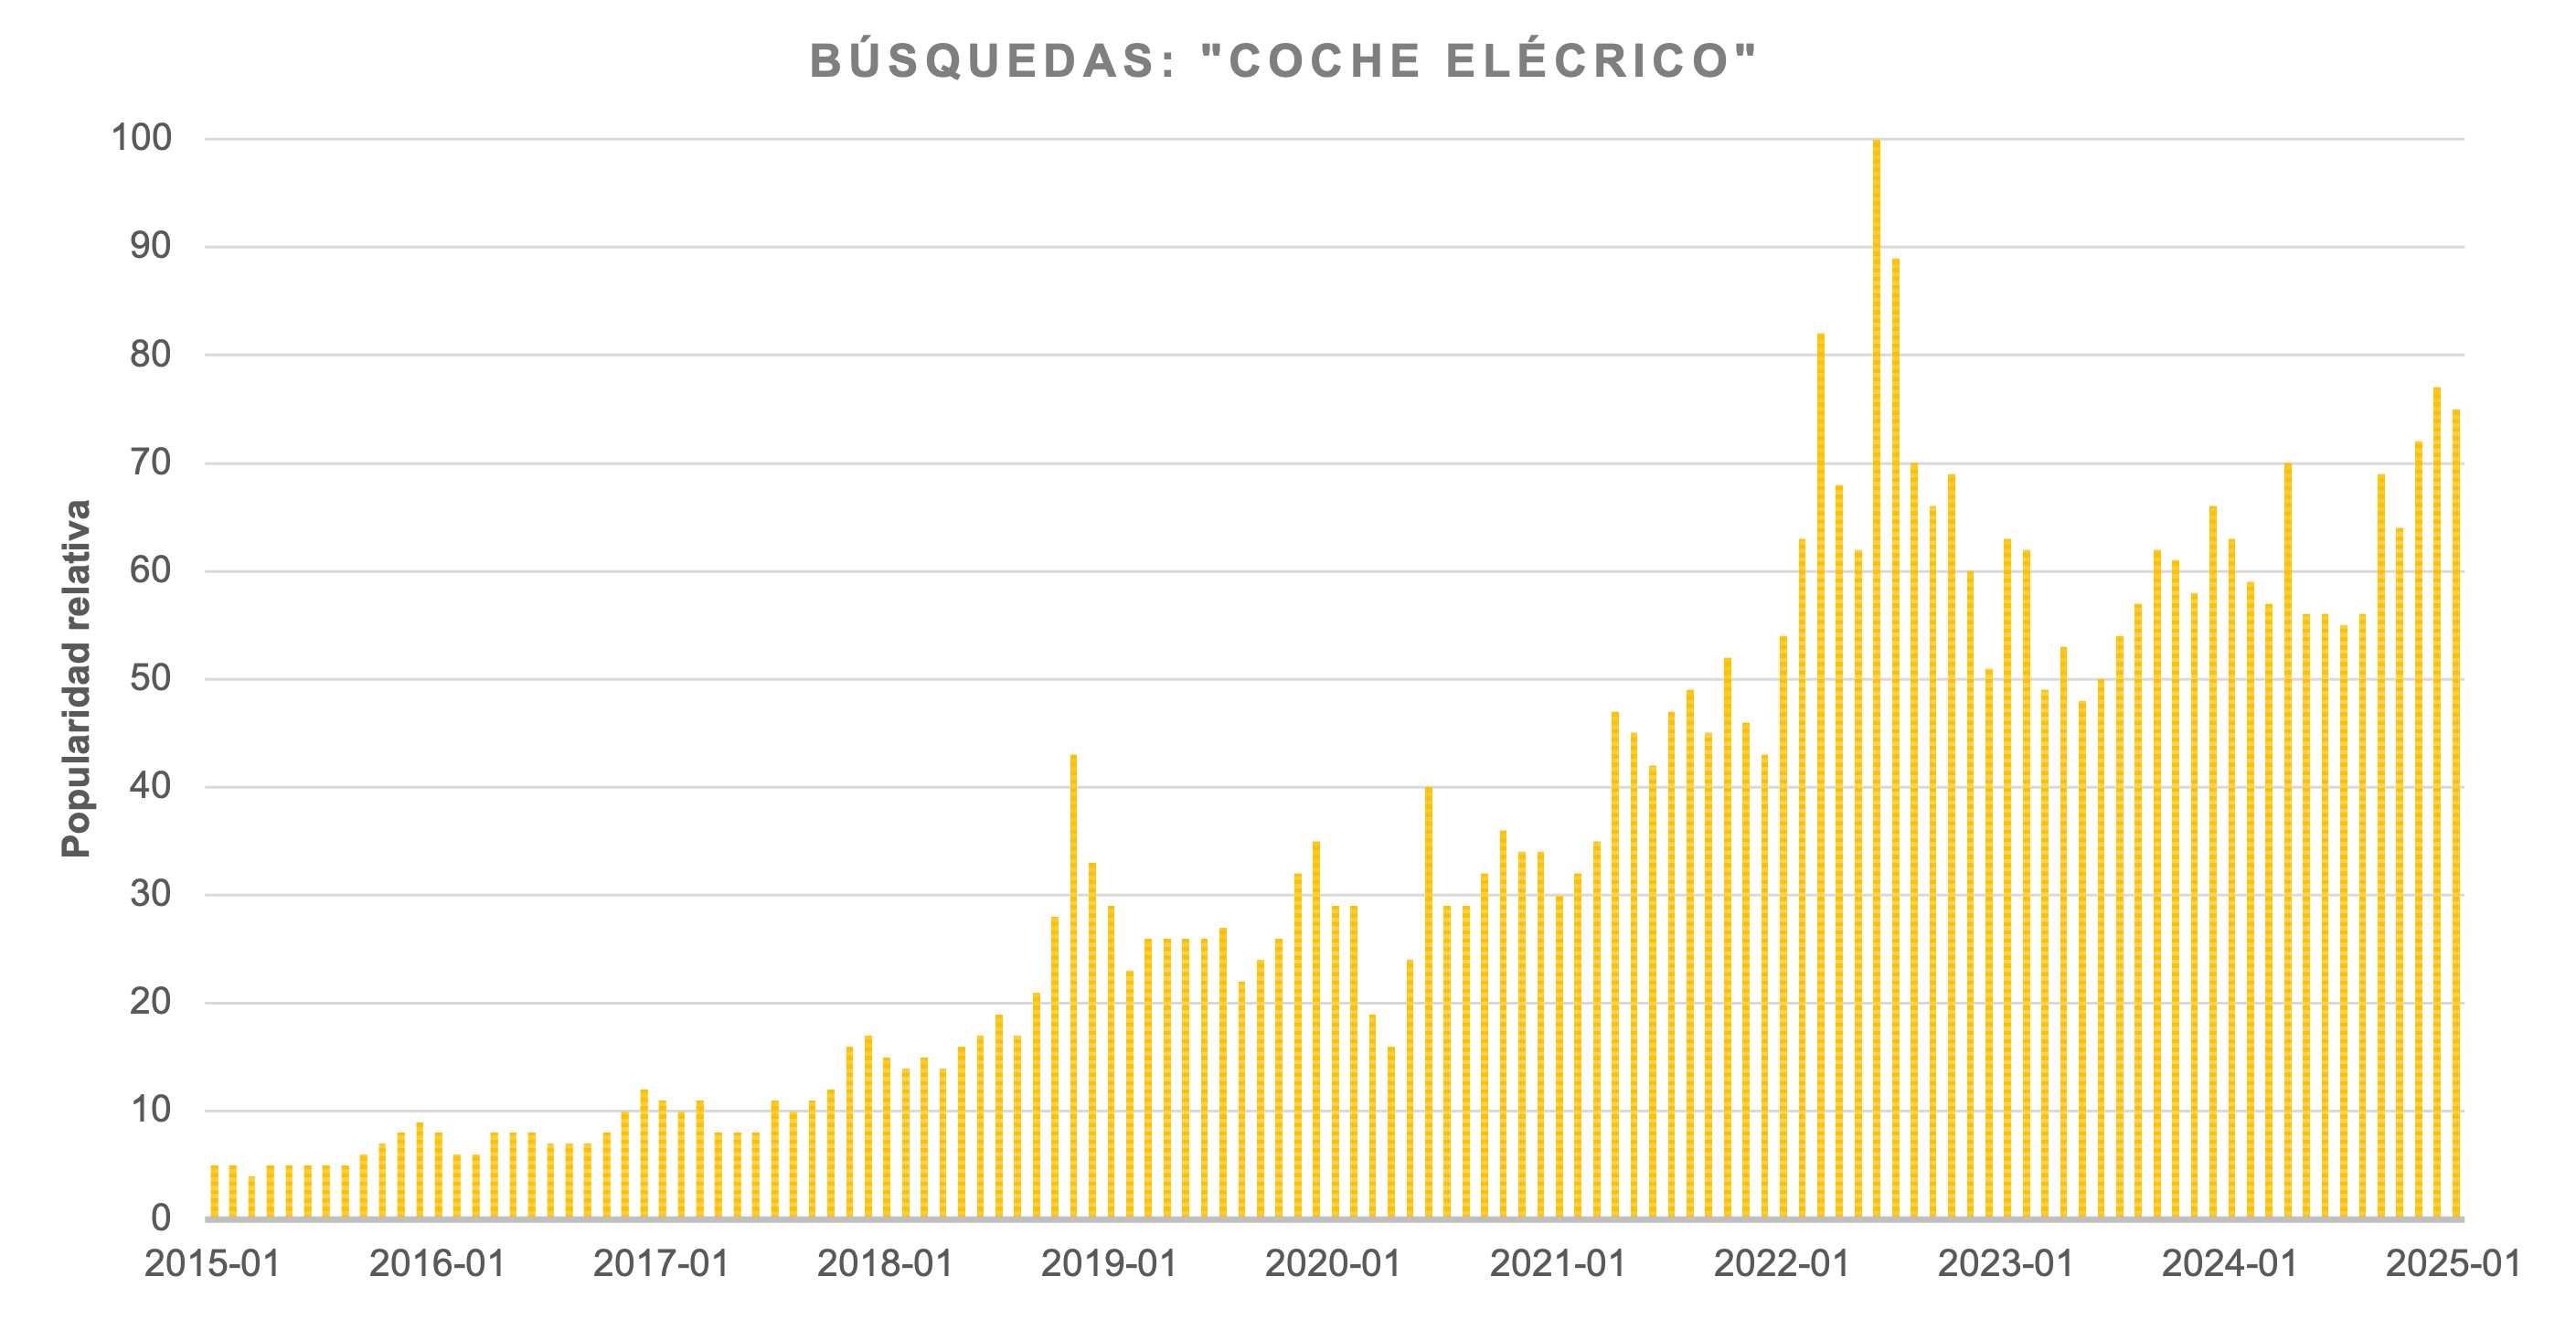
\includegraphics[width=1\textwidth]{images/EV_search_graph.png}
    \caption{Evolución del interés por los vehículos eléctricos en España (2015-2025). 
    Fuente: Google Trends~\cite{googletrends2025}}
    \label{fig:ev_interest}
\end{figure}

Además, la variabilidad en la disponibilidad de energía renovable, como la solar y la eólica,
las fuentes renovables más populares en nuestro país%\cite{kim2024renewable}
, introduce 
incertidumbre en la generación de energía. Esto, a su vez, requiere una gestión más dinámica 
y flexible de la demanda para garantizar un suministro estable y eficiente. La gestión de la 
carga de los vehículos eléctricos es un aspecto crítico para garantizar que la transición hacia 
un sistema de transporte sostenible no comprometa la estabilidad de la red eléctrica.\\

La Inteligencia Artificial Generativa (IA Generativa) surge como una herramienta
prometedora para enfrentar estos desafíos. Gracias a su capacidad de analizar grandes
volúmenes de datos en tiempo real, la IA Generativa puede predecir patrones de consumo,
optimizar la generación y distribución de energía, anticipar fallos en infraestructuras y
ajustar el consumo a las condiciones de la red de manera más eficiente y eficaz que los métodos
tradicionales.\\

La IA Generativa permite la creación de modelos predictivos que pueden simular diferentes
perfiles de carga, facilitando la toma de decisiones informadas y la implementación de estrategias
de gestión de la demanda más efectivas. Además, su capacidad para aprender y adaptarse a nuevas 
condiciones y entornos, la convierte en una herramienta valiosa para la planificación y operación 
de sistemas energéticos cada vez más complejos.

\section{Motivación}
La gestión responsable y eficiente de la energía es una tarea de vital importancia para una 
sociedad cada día más consciente y proactiva en tareas de sostenibilidad. Añadiendo a este panorama
el crecimiento experimentado por la movilidad eléctrica en el siglo XXI, dicha gestión eficiente y 
responsable del consumo energético aplica necesariamente a la carga de vehículos eléctricos.\\

La carga de estos vehículos puede generar picos de demanda que, si no se gestionan adecuadamente, 
pueden comprometer la fiabilidad de la red eléctrica y aumentar los costes operativos, 
repercutiendo finalmente en los consumidores. Además, la variabilidad en la disponibilidad de 
energía renovable, como la solar y la eólica, introduce incertidumbre en la generación de energía, 
lo que requiere una gestión más dinámica y flexible de la demanda para garantizar un suministro 
estable y eficiente.\\

Las innovadoras herramientas que presenta la IA Generativa, junto con las redes neuronales 
(Neural Networks, NN) basadas en aprendizaje por refuerzo (Reinforcement Learning, RL), exhiben 
un gran potencial para abordar estos retos de manera novedosa, y con resultados del más alto 
rendimiento.

\section{Objetivos}
El objetivo del proyecto es desarrollar in sistema gestor inteligente para la carga de EVs en un 
contexto dómestico. Para ello, se hará uso de técnicas de IA Generativa, RLNN (Reinforcement 
Learning Neural Network) y algoritmos clásicos de optimización.\\

El gestor deberá decidir, en base a una serie de restricciones y requisitos, tanto físicos como 
lógicos, si cargar o no el EV en un momento dado. Idealmente, el gestor conseguirá cargar el EV 
de la forma más eficiente posible, minimizando el coste de la carga y maximizando el uso de energía
disponible, al tiempo que se cumplen las restricciones impuestas por el usuario y las 
características del sistema eléctrico.\\

Para lograr este objetivo, se han definido unos objetivos secundarios específicos. El primero tiene
que ver con toda la parte generativa del proyecto: la creación de perfiles sintéticos de demanda no
gestionable, disponibilidad y requisitos del EV. En segundo lugar,se realizará una optimización 
clásica, tratando el problema de la carga como un pograma lineal (Linear Programme, LP), y se 
resolverá como tal. Con esta optimización clásica, que garantiza un resultado óptimo según las 
restricciones que se le impongan en forma de ecuación, se compararán los resultados de ambos 
métodos.\\

Se evaluarán tres métricas principales: coste incurrido en la carga, cuantía de energía empleada y 
rendimiento computacional.

\section{Estructura}
El trabajo está estructurado en seis capítulos, incluyendo este introductorio. Tras esta breve 
introducción, exposición de la motivación para el proyecto y los objetivos que se pretenden 
alcanzar, el segundo capítulo se centra en la revisión del estado del arte, donde se analizarán las 
técnicas de IA Generativa, las redes neuronales con aprendizaje por refuerzo y su aplicación en la 
gestión de la demanda energética.\\

El tercer capítulo presenta el diseño y desarrollo del sistema propuesto, incluyendo la 
arquitectura de la red neuronal y el enfoque de aprendizaje por refuerzo utilizado. Es decir, la 
metodología llevada a cabo durante el proyecto. El cuarto capítulo ofrece una explicación 
detallada de la implementación del sistema de acuerdo a lo explicado en el estado del arte, y 
contenido en el marco de la metodología. En este capítulo se detallan los algoritmos
implementados, las técnicas de IA Generativa utilizadas y la forma en que se integran para
lograr los objetivos del proyecto.\\

El quinto capítulo muestra una discusión de la comparación de los resultados obtenidos con los
diferentes enfoques - la optimización clásica y el sistema de RLNN + IAGen - y una evaluación 
de su rendimiento en términos de coste, eficiencia y rendimiento computacional. Finalmente, en
el sexto capítulo se presentan las conclusiones del proyecto, así como las posibles líneas de
investigación futura. Se reflexiona sobre los logros alcanzados, las lecciones aprendidas y
las implicaciones de los resultados obtenidos. Además, se discuten las posibles aplicaciones
prácticas del sistema desarrollado, dando fin al proyecto.\\ 

El trabajo se complementa con una serie de apéndices que incluyen detalles técnicos adicionales,
enlace al código fuente y otros materiales relevantes que respaldan la investigación y el 
desarrollo. Estos apéndices proporcionan una visión más profunda de los aspectos técnicos
del proyecto y permiten una comprensión más completa de los métodos y resultados presentados.

\vfill
 % This is the way we should import files and partition our document.
	\cleardoublepage
	\chapter{Estado del Arte}
\section{Fuentes de datos}
Tal y como se ha explicado en la intriducción, durante el desarrollo del proyecto se van a combinar
técnicas de IA Generativa, Redes Neuronales con Aprendizaje por Refuerzo y algoritmos clásicos de 
optimización. Para ello, es necesario tener acceso a distintas fuentes de datos, que se adapten
a cada una de las técnicas que se van a utilizar.\\

De acuerdo con los objetivos propuestos, y el planteamiento general del proyecto, las fuentes de 
datos para este proyecto son las dos siguientes:
\begin{itemize}
    \item \textbf{Electric Vehicle Charging Patterns Dataset}
    \item \textbf{Load Profile Generator}
\end{itemize}

\subsection{Electric Vehicle Charging Patterns Dataset}
\textit{Electric Vehicle Charging Patterns} es un conjunto de datos obtenidoo desde la plataforma
\textit{Kaggle}~\cite{kaggle_ev_charging_patterns}, que contiene información sobre los patrones de 
carga de vehículos eléctricos (EVs) en un entorno urbano. Tal y como lo describe su autor, "otorga 
un análisis exhaustivo de patrones de carga de EVs y comportamiento de los usuarios". El dataset 
incluye 1320 muestras sobre el consumo energético durante la carga, la duración de la carga y 
detalles de cada uno de los vehículos registrados, de entre sus 20 campos.\\
\vfill
\begin{table}[ht]
\begingroup
\centering
\setlength{\tabcolsep}{6pt}
\begin{tabular}{c|l c c c}
 & Modelo & Capacidad (kWh) & SoC Inicial (\%) & SoC Final (\%) \\
\hline
0 & BMW i3 & 108.46 & 29.37 & 86.12 \\
1 & Hyundai Kona & 100.00 & 10.12 & 84.66 \\
2 & Chevy Bolt & 75.00 & 6.85 & 69.92 \\
3 & Hyundai Kona & 50.00 & 83.12 & 99.62 \\
4 & Hyundai Kona & 50.00 & 54.26 & 63.74 \\
\end{tabular}
\caption{Pequeña muestra de los datos del dataset \textit{Electric Vehicle Charging Patterns}.}
\label{tab:ev_charging_patterns_example}
\endgroup
\end{table}

\subsection{Load Profile Generator}
\textit{Load Profile Generator} es una aplicación desarrollada por Noah Pflugradt, de la 
\textit{Bern University of Applied Sciences}~\cite{pflugradt2020loadprofile}
, que genera perfiles de carga sintéticos para un hogar, incluyendo la demanda de energía 
no gestionable, la disponibilidad de carga y los requisitos del vehículo eléctrico. Este 
generador es capaz de crear perfiles de carga sintéticos que simulan el comportamiento 
real de un hogar, lo que permite entrenar y evaluar modelos de IA sin necesidad de datos 
reales.
\begin{figure}[ht]
    \centering
    \includegraphics[width=0.75\textwidth]{images/lpg_logo.png}
    \caption{Logo de LPG. Fuente: \textit{LoadProfileGenerator}~\cite{pflugradt2020loadprofile}.}
    \label{fig:lpg_logo}
\end{figure}

Esta herramienta ha sido instrumental para el desarrollo del proyecto, permitiendo la generación
de consumos completamente realistas, en una amplia variedad de escenarios predefinidos. La 
personalización para la generación de los datos dentro del progama permite generar consumos para
diferentes configuraciones de hogares, variando el número de hijos, su actividad física, la 
distancia al trabajo y muchas más opciones.\\

Además de la variabilidad, en cuanto al análisis de datos se refiere, no sólo facilita el
procesado de los datos, devolviendo los resultados en CSVs (Comma Separated Values) agrupados con 
el consumo global, y también separando por tipos de consumo; sino que el propio programa permite el
ajuste granulado de la resolución temporal interna y externa. De manera que los datos que se han 
generado y se usan en este proyecto, tienen una resolución interna de un minuto, y una resolución 
externa de 15 minutos.

\begin{figure}[ht]
    \centering
    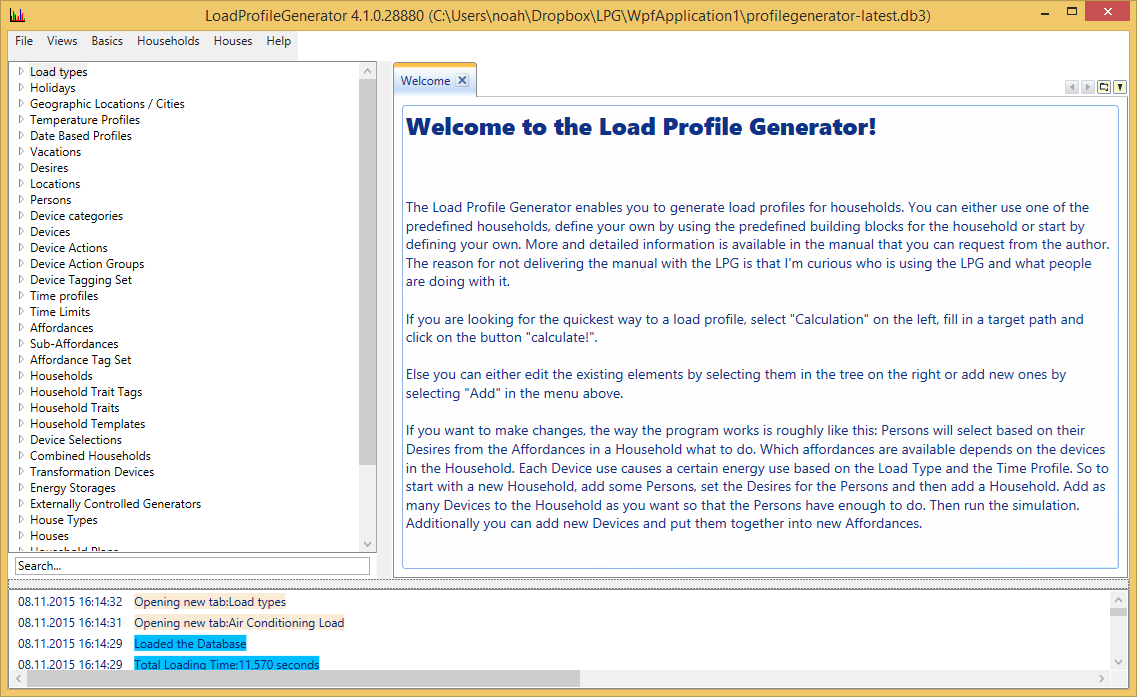
\includegraphics[width=0.7\textwidth]{images/LPG_screenshot.png}
    \caption{Capturas de pantalla de LPG, página principal. 
    Fuente: \textit{LoadProfileGenerator}~\cite{lpg_screenshots_2025}.}
    \label{fig:lpg_screenshot}
\end{figure}
\begin{figure}[ht]
    \centering
    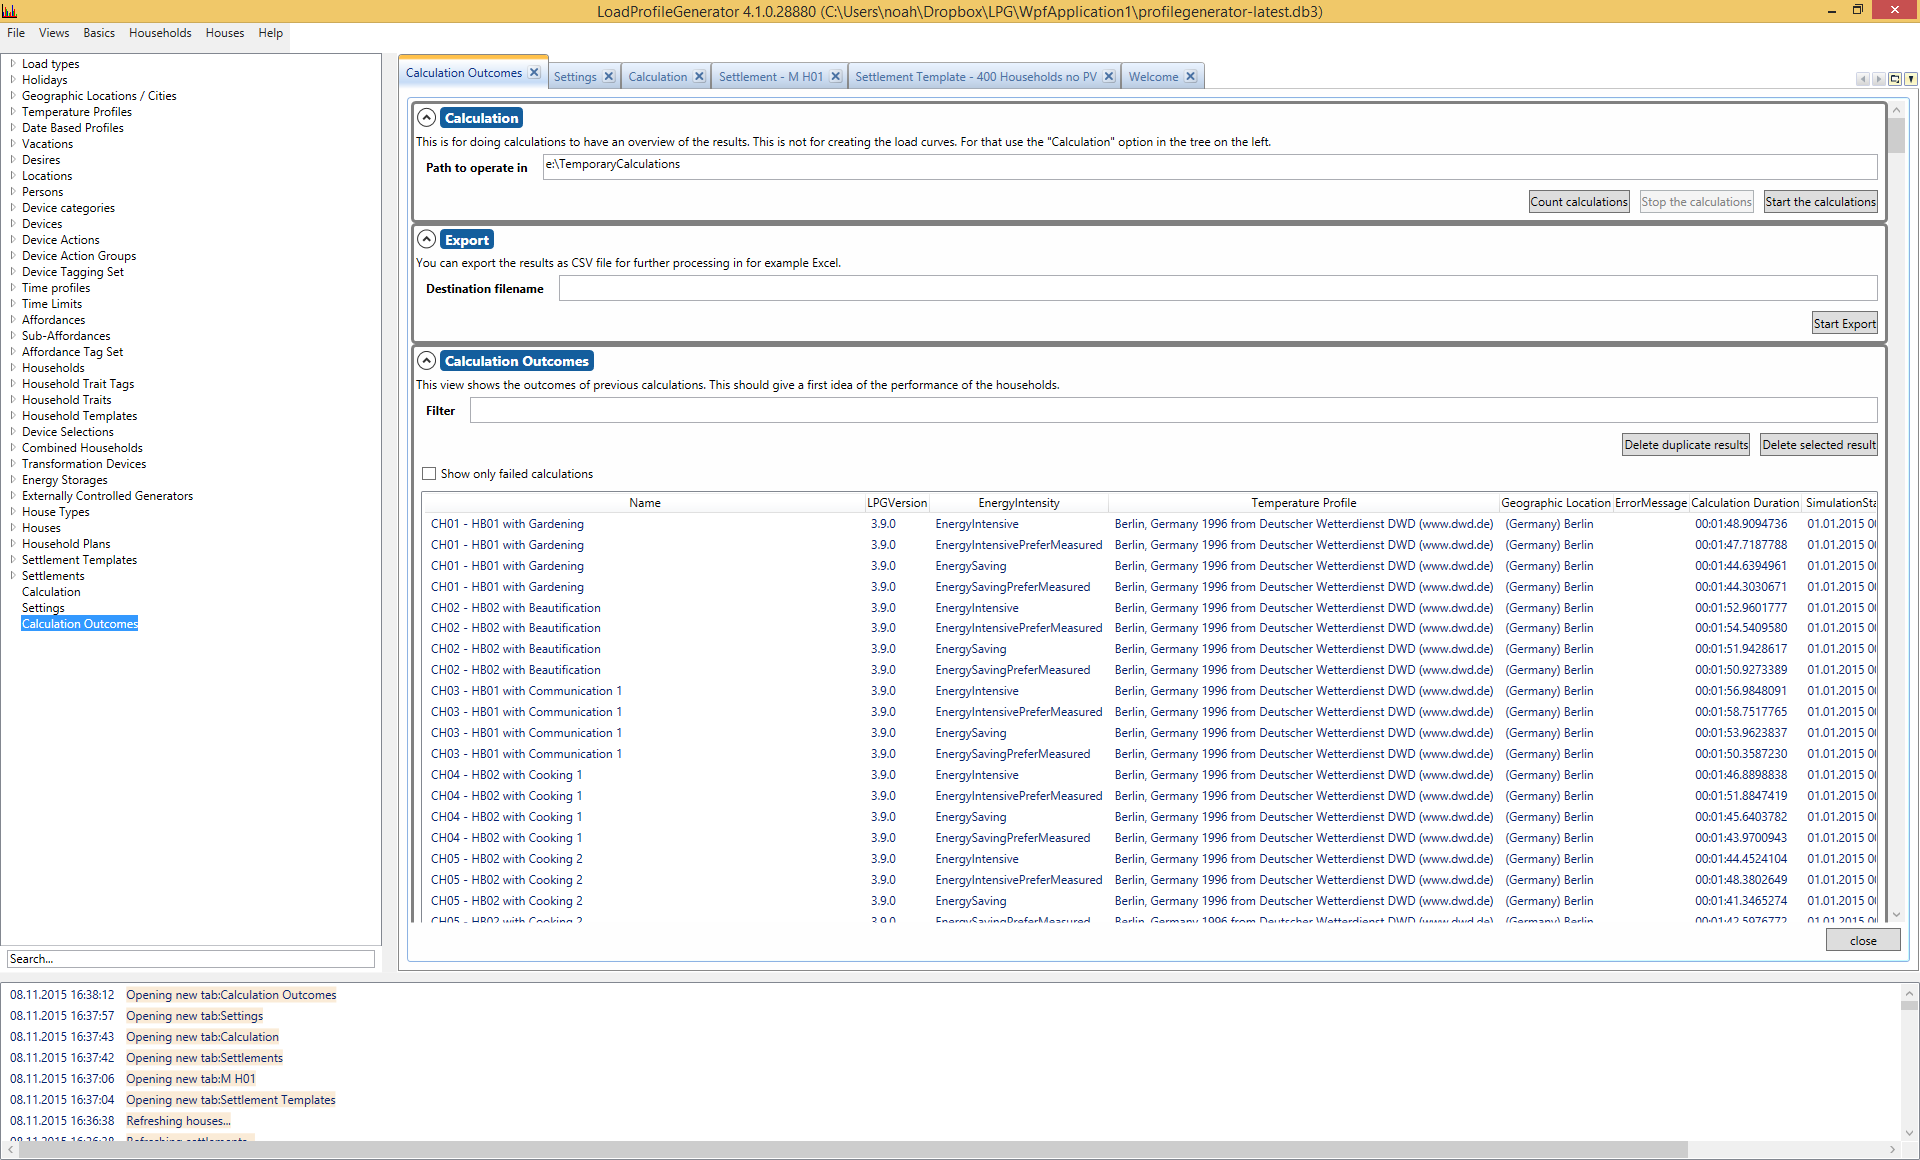
\includegraphics[width=0.7\textwidth]{images/LPG_screenshot_2.png}
    \caption{Capturas de pantalla de LPG, obtención de resultados. 
    Fuente: \textit{LoadProfileGenerator}~\cite{lpg_screenshots_2025}.}
    \label{fig:lpg_screenshot2}
\end{figure}

\section{Optimización Clásica}
La optimización clásica, o programación matemática, es el conjunto de métodos, principios y 
técnicas que se utilizan para encontrar la mejor solución a un problema cuantitativo concreto, 
sujeto a un conjunto de restricciones o condiciones, que limitan el conjunto de soluciones posibles~\cite{wright2025optimization}.
En su forma más básica, la optimización clásica busca maximizar o minimizar una función real, 
referida como función objetivo, resolviendo una serie de ecuaciones y/o desigualdades. Por tanto,
se puede definir la optimización como la elección del mejor elemento dentro de una selección de 
elementos disponibles, sujetos a algún criterio~\cite{wikipedia2025optimizacion}.\\

La optimización clásica se divide en varias categorías, dependiendo de la naturaleza de la función
objetivo y las restricciones. Las categorías más comunes son:
\begin{itemize}
    \item \textbf{Programación Lineal}
    \item \textbf{Programación Entera}
    \item \textbf{Programación No Lineal}
\end{itemize}

\subsection{Programación Lineal}
La programación lineal es un caso concreto del espacio de métodos recogido bajo el término 
\textit{Programación Convexa}. Este concepto se refiere a los programas que resuelven problemas 
en los que la función objetivo es cóncava (maximización) o convexa (minimización). Dentro de este
marco, la programación lineal es el caso particular en el que la función objetivo y las restricciones
son ecuaciones o inecuaciones estrictamente lineales~\cite{wikipedia2025optimizacion}.\\

Geométricamente, puede ser interpretado como si dichas restricciones definieran una figura en el 
espacio euclídeo, y la función objetivo es la dirección en la que se busca maximizar o minimizar el 
valor de la función~\cite{funke2024discreteopt}. Un ejemplo de un problema de programación lineal 
es el siguiente:
\begin{align*}
    \text{Max.} \quad & z = 3x + 2y \\
    \text{Sujeto a} \quad & x + y \leq 4 \\
    & 2x + y \leq 6 \\
    & x \geq 0, \quad y \geq 0
\end{align*}

Aquí, la función objetivo es \(z = 3x_1 + 2x_2\), y las restricciones son claramente lineales. El
objetivo es encontrar los valores de \(x_1\) y \(x_2\) tal que \(z\) sea máxima mientras se cumplen 
las restricciones. La solución óptima se puede encontrar utilizando el método simplex o el método 
de interior-puntos, entre otros algoritmos de optimización lineal~\cite{wikipedia2025optimizacion}.

\subsection{Programación Entera}
Este tipo de programación analiza programas lineales en los que se fuerza que, al menos una de las 
variables, esté forzada a ser un número entero. En este caso particular, la programación entera se
aleja de la programación convexa, ya que la función objetivo y las restricciones no son 
estrictamente lineales, y su resolución suele resultar más compleja que la de un programa lineal 
al uso~\cite{wikipedia2025optimizacion}. La programación entera se divide en dos categorías:
\begin{itemize}
    \item \textbf{Programación Entera \textit{Mixta} (MIP)}: En este caso, algunas variables son enteras y
    otras pueden tomar valores continuos. Este tipo de programación es muy común en problemas de
    optimización combinatoria, donde se busca una solución óptima entre un conjunto discreto de
    opciones, como la asignación de recursos o la planificación de rutas. Hay casos en los que las
    variables pueden tomar valores continuos dentro de un número de opciones discreto, por ejemplo: 
    [0, 0.5, 1] \cite{funke2024discreteopt}.
    \item \textbf{Programación Entera \textit{Pura} (IP)}: En este caso, todas las variables son enteras.
    Este tipo de programación se utiliza en problemas donde todas las decisiones deben ser discretas,
    como la selección de proyectos o la asignación de tareas \cite{funke2024discreteopt}.
\end{itemize}

\subsection{Programación No Lineal}
Como dice su nombre, la programación no lineal es el caso en el que la función objetivo y/o las
restricciones no son lineales \cite{wikipedia2025optimizacion}. Este tipo de programación es más
complejo que la programación lineal, ya que las funciones no lineales pueden tener múltiples
mínimos o máximos locales, lo que dificulta la búsqueda de la solución óptima. Además, la
programación no lineal puede involucrar todo tipo de funciones: cuadráticas, exponenciales, 
logarítmicas o trigonométricas, entre otras \cite{funke2024discreteopt}.

\section{Aprendizaje por Refuerzo (RL)}
Stutton y Barto definen el Aprendizaje por Refuerzo (Reinforcement Learning, RL) como un
"enfoque de aprendizaje automático en el que un agente aprende a tomar decisiones mediante la
interacción con un entorno, recibiendo recompensas o penalizaciones en función de sus acciones".
En otras palabras, RL es aprender qué hacer, asociar situaciones con acciones, para maximizar una
recompensa numérica~\cite{sutton2018reinforcement}.\\

Es importante resaltar la diferencia entre el Aprendizaje Supervisado y el Aprendizaje por Refuerzo. 
En el primer caso, el modelo aprende a partir de un conjunto de datos etiquetados, donde cada 
entrada tiene una salida conocida. En el caso del Aprendizaje por Refuerzo, el modelo aprende a 
partir de su propia experiencia, obtenida tras una serie de interaccioens con el entorno. Por lo 
mismo, el RL es también diferente a lo comúnmente conocido como \textit{Aprendizaje no Supervisado}, 
ya que este grupo de métodos típicamente buscan patrones o estructuras en una colección de datos sin
etiquetar~\cite{sutton2018reinforcement}.\\

Un problema único para los algoritmos de aprendizaje por refuerzo es el equilibrio entre 
exploración y explotación - o \textit{exploration-exploitation trade-off} -. El término exploración
suele hacer referencia a la "curiosidad" del agente por encontrar nuevas y diferentes estrategias,
mientras que explotación se refiere a la tendencia del agente a explotar las estrategias que ya
concoe, y sabe que otorgan resultados positivos. Encontrar un equilibrio balanceado entre estas 
dos características es tremendamente importante para conseguir el aprendizaje posible del agente
\cite{sutton2018reinforcement}.

\subsubsection{Glosario de términos clave en Aprendizaje por Refuerzo}

Tras una breve introducción al Aprendizaje por Refuerzo, es importante definir algunos de los
términos clave que se utilizan en este campo. Estos términos son fundamentales para entender
los conceptos y algoritmos que se desarrollan en el ámbito del RL. A continuación, se presentan
los términos más relevantes y que serán utilizados a lo largo del trabajo:
\cite{wang2022nn_drl}
\begin{itemize}
    \item \textbf{Agente}: Es la parte que toma decisiones y ejecuta acciones dentro del entorno, 
    con el objetivo de maximizar su recompensa acumulada.
    \item \textbf{Acción (A)}: Conjunto de todas las posibles acciones que el agente puede 
    realizar en un estado dado. Una acción concreta se denota habitualmente como \(a\).
    \item \textbf{Factor de descuento (\(\gamma\))}: Parámetro que determina la importancia de las 
    recompensas futuras frente a las inmediatas. Un valor bajo de \(\gamma\) resulta en un agente
    cortoplacista. En caso contrario, el agente tendrá una visión más global y a largo plazo.
    \item \textbf{Estado (S)}: El contexto instantáneo en que se encuentra el agente en cualquier 
    momento.
    \item \textbf{Entorno}: Es el "mundo" en el que opera el agente. Recibe como entrada el estado 
    actual y la acción seleccionada, y devuelve la recompensa obtenida y el nuevo estado resultante.
    \item \textbf{Recompensa (r)}: Retroalimentación que recibe el agente tras ejecutar una acción 
    en un estado determinado. Indica el grado de éxito o fracaso de la acción tomada.
    \item \textbf{Política (\(\pi\))}: Estrategia que sigue el agente para decidir qué acción tomar 
    en cada estado. %Formalmente, es una función que asigna a cada estado la acción que maximiza la recompensa esperada.
    \item \textbf{Valor (V)}: Valor esperado de la recompensa acumulada (a largo plazo y con 
    descuento) que puede obtener el agente desde un estado concreto, siguiendo una política 
    determinada.
    \item \textbf{Valor de acción (Q)}: Valor esperado de la recompensa acumulada (con descuento) 
    que puede obtener el agente al tomar una acción específica en un estado dado, y siguiendo 
    posteriormente una política determinada. Es la función que asigna pares estado-acción a 
    recompensas esperadas.
\end{itemize}

\subsection{Redes Neuronales dentro del RL}
Al final, en un algoritmo de RL, un entorno es una función que transforma una acción en el 
siguiente estado y recompensa, y los agentes son funciones que transforman la función de 
recompensa y el estado en la siguiente acción. Es aquí donde las redes neuronales entran en juego, 
ya que, en esencia, no son más que aproximadores de funciones.\\

Por esta condición de aproximadores de funciones que presentan las redes neuronales, son una 
herramienta excelente cuando el conjunto de acciones y/o de estados es demasiado grande, o no del
todo conocido, siendo este el caso de la inmensa mayoría de los casos de uso en el mundo real.
En estos casos, las redes neuronales pueden aprender a aproximar la función de valor o la política
del agente, permitiendo que el agente tome decisiones informadas basadas en la información
disponible \cite{wang2022nn_drl}.\\

Una RLNN, por ejemplo, puede ser la solución idónea para una IA que aprenda a jugar al ajedrez. El
ajedrez es el juego de estrategia por excelencia, y es tan complejo que no es posible enumerar 
todas las posibles jugadas y resultados. Por tanto, una RLNN puede aprender a jugar al ajedrez a 
través de la experiencia, jugando millones de partidas y ajustando su política de juego en función 
de las recompensas obtenidas al término de cada movimiento o cada partida.

\begin{figure}[ht]
    \centering
    
\includegraphics[width=0.65\textwidth]{images/DeepMind_new_logo.svg.png}
    \caption{Logo de DeepMind. Fuente: DeepMind \cite{deepmind2025website}.}
    \label{fig:deepmind_logo}
\end{figure}

Alpha Zero, la IA desarrollado por Google DeepMind, utiliza una red neuronal con aprendizaje por 
refuerzo, y ha aprendido a jugar al ajedrez, al Go y al shogi con un novel tal, que ha sido capaz
de superar a los mejores jugadores humanos y por supuesto a otros programas de ajedrez, gracias a 
su capacidad para aprender, después de millones de partidas, y adaptarse a diferentes estilos de 
juego \cite{deepmind2017alphazero}.

\subsection{Deep Q-Networks (DQN)}
Una \textit{Deep Q-Network} (DQN) es uno de los algoritmos más potentes y populares en RL, ya que 
hace uso de la combinación de redes neuronales profundas y \textit{Q-Learning}, permitiendo al
agente aprender políticas tremendamente omtimizadas en entornos muy complejos. \cite{dhumne2019dqn}.

\begin{figure}[ht]
    \centering
    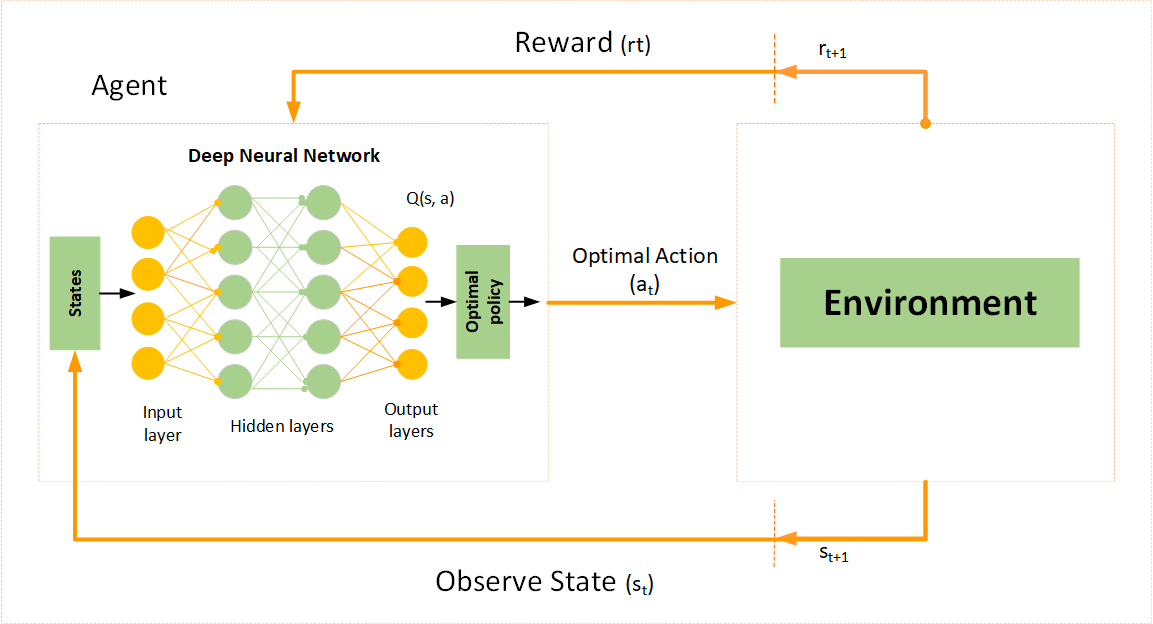
\includegraphics[width=0.9\textwidth]{images/image.png}
    \caption{Arquitectura general de una Deep Q-Network (DQN). Fuente: Deep Q-Learning (DQN)
    \cite{amin2020dqn}.}
    \label{fig:dqn_architecture}
\end{figure}

\textit{Q-Learning} es un algoritmo que enseña a los agentes a comportarse de manera óptima en un 
entorno Markoviano controlado, esto es un entorno en el que la probabilidad de transición entre 
estados depende únicamente del estado actual y la acción tomada, y no de estados anteriores. 
Funciona mejorando iterativamente la evaluación de una acción específica en un estado determinado
\cite{watkins1992qlearning}.

\subsubsection{Funcionamiento de DQN \cite{mnih2013dqn}}
El algoritmo Deep Q-Network (DQN) es una técnica de aprendizaje por refuerzo que utiliza redes 
neuronales para aprender a tomar decisiones. En lugar de trabajar con tablas de valores como el 
Q-learning tradicional, DQN usa una red para aproximar los valores \( Q(s, a) \), que indican lo 
buena que es una acción \( a \) en un estado \( s \).

\begin{itemize}
    \item \textbf{Valor objetivo:} Para aprender, DQN compara su predicción con un valor objetivo,
    calculado como:
    \[
    y = r + \gamma \max_{a'} Q(s', a'; \theta^-)
    \]
    donde:
    \begin{itemize}
        \item \( r \) es la recompensa obtenida tras hacer una acción,
        \item \( s' \) es el siguiente estado,
        \item \( \gamma \) es un número entre 0 y 1 que da más o menos importancia a las recompensas 
        futuras,
        \item \( \theta^- \) son los parámetros de una copia de la red (llamada red objetivo).
    \end{itemize}

    \item \textbf{Función de pérdida:} La red aprende minimizando la diferencia entre lo que predice 
    y el valor objetivo:
    \[
    L(\theta) = \mathbb{E}_{(s, a, r, s') \sim D} \left[ \left( y - Q(s, a; \theta) \right)^2 \right]
    \]
    Aquí, \( D \) es un conjunto de experiencias almacenadas (replay buffer), que permite entrenar de 
    forma más estable y variada.

    \item \textbf{Entrenamiento:} Los parámetros \( \theta \) de la red se actualizan usando un 
    algoritmo de optimización (como descenso de gradiente) que intenta reducir el error en las 
    predicciones.

    \item \textbf{Red objetivo:} Para evitar que el entrenamiento sea inestable, DQN usa una segunda 
    red (la red objetivo) que se mantiene fija durante varios pasos y se actualiza solo cada cierto 
    tiempo copiando los valores de la red principal.
\end{itemize}

\subsubsection{Ventajas de DQN \cite{dhumne2019dqn}}
\begin{itemize}
    \item[(+)] El uso de redes neuronales profundas otorga a DQN la capacidad de aprender 
    representaciones abstractas y de alta dimensionalidad, facilitando el aprendizaje en entornos 
    complejos.
    \item[(+)] La utilización de un \textit{replay buffer} permite un entrenamiento más estable y 
    eficiente, ya que el agente puede revisar experiencias pasadas y no depende únicamente de las 
    más recientes.
    \item[(+)] DQN tiene una gran capacidad de generalización, permitiéndole desenvolverse en 
    situaciones no vistas previamente, lo que lo hace muy adecuado para problemas de RL complejos.
\end{itemize}

\subsubsection{Inconvenientes de DQN \cite{dhumne2019dqn}}
\begin{itemize}
    \item[(-)] DQN es sensible a la elección de hiperparámetros, como la tasa de aprendizaje, el 
    factor de descuento, el ratio de exploración y el tamaño del \textit{replay buffer}, lo que 
    puede afectar significativamente su rendimiento.
    \item[(-)] No está diseñado para su uso en línea, siendo más adecuado para entornos 
    \textit{offline}.
    \item[(-)] La actualización de \textit{Q-learning} implementada en DQN puede ser propensa a la 
    sobreestimación de los valores \( Q \).
\end{itemize}

\subsection{Long Short-Term Memory (LSTM)}
Las redes \textit{Long Short-Term Memory} (LSTM) son una arquitectura de redes neuronales 
recurrentes (RNNs) diseñada para gestionar información secuencial de forma más eficaz. A diferencia 
de las RNN simples, que utilizan un único vector oculto para propagar información, las LSTM 
incorporan una estructura interna más compleja que les permite mantener información relevante 
durante más tiempo y decidir qué conservar y qué olvidar~\cite{bulling2024rnn}.

\begin{figure}[ht]
    \centering
    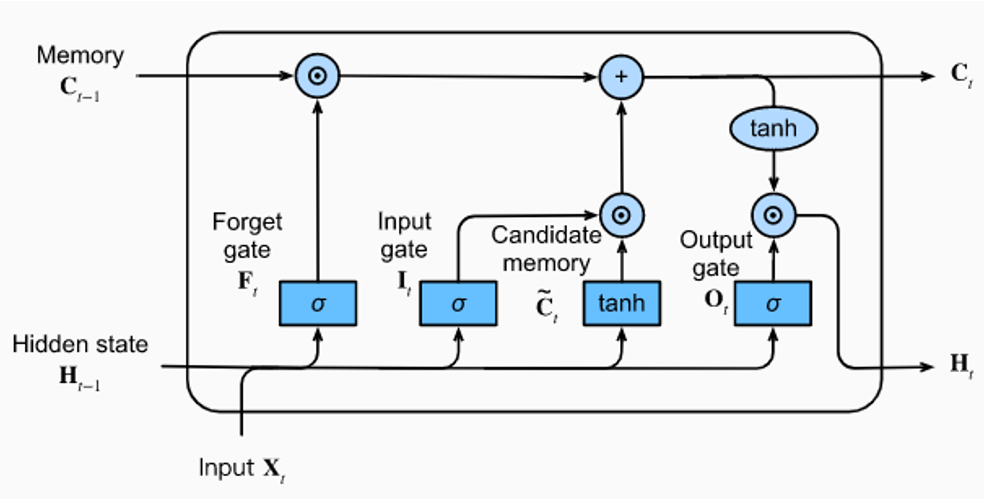
\includegraphics[width=0.8\textwidth]{images/LSTM_diagram.png}
    \caption{Diagrama LSTM. Fuente: \textit{An Intuitive Explanation of LSTM}~\cite{calzone2020lstm}.}
    \label{fig:lstm_diagram}
\end{figure}

Internamente, una LSTM introduce tres puertas: la \textit{puerta de entrada}, la 
\textit{puerta de olvido} y la \textit{puerta de salida}. Estas puertas actúan como filtros que 
controlan el flujo de información a lo largo del tiempo:
\begin{itemize}
    \item La puerta de entrada determina qué parte de la información nueva debe almacenarse.
    \item La puerta de olvido decide qué parte del contenido anterior debe descartarse.
    \item La puerta de salida regula qué información del estado interno se transmite a la 
    siguiente capa o paso de tiempo.
\end{itemize}

Gracias a esta estructura, las LSTM son especialmente útiles para tareas donde es importante 
tener en cuenta el contexto anterior, como el procesamiento de lenguaje natural, la clasificación 
de secuencias o la predicción de series temporales. La capacidad de decidir dinámicamente qué 
recordar y qué olvidar convierte a las LSTM en una herramienta eficaz para trabajar con 
dependencias temporales prolongadas \cite{calzone2020lstm}. Estas propiedades hacen que las LSTM 
sean más robustas para modelar dependencias a largo plazo en secuencias, en comparación con las RNN 
simples.

\section{Técnicas de IA Generativa}
A lo largo de esta sección, se tratará de explicar y exponer las principales técnicas usadas en el
mundo de la inteligencia artificial generativa, que pueden trasladarse de manera práctica al 
sector eléctrico. Las cuatro técnicas que tratar son:

\begin{itemize}
    \item \textbf{Generative Adversarial Networks (GANs)}
    \item \textbf{Variational Autoencoders (VAEs)}
    \item \textbf{Modelos de difusión}
    \item \textbf{Modelos fundacionales}
\end{itemize}

\subsection{Generative Adversarial Networks (GANs)}
Esta primera técnica, emplea aprendizaje no supervisado con dos redes neuronales contrapuestas. 
Éstas, son entrenadas de manera que compiten entre sí, en un proceso similar a un juego de “suma 
cero”.\\

Durante el entrenamiento, una de las dos redes, la red A, genera candidatos para ser evaluados por 
la red B. Normalmente, la red A se entrena para que genere candidatos y estímulos siguiendo una 
determinada distribución o reglas, mientras que la red B pretende discriminar y diferenciar casos 
originales de casos generados artificialmente.\\

Con este planteamiento, el objetivo es complicarle la tarea a la red B, consiguiendo que el output 
de la red A sea tan similar al original, que dificulte la diferenciación. \cite{xiao2022gan}.

\begin{table}[H]
\centering
\begin{tabularx}{\textwidth}{X|X}
    \textbf{Fortalezas} & \textbf{Debilidades} \\ \hline
    Generación de imágenes & Entrenamiento complejo \\ 
    Reescalado & Inestabilidad y ``mode collapse'' \\
    Multimodalidad & \\ 
    Gran versatilidad & \\ 
\end{tabularx}
\caption{Fortalezas y debilidades de las GANs}
\end{table}

\subsection{Variational Autoencoders (VAEs)}
El segundo tipo de modelo generativo, los Autocodificadores Variacionales, son modelos que aprenden 
de sus datos como una representación comprimida de los mismos, asignados a una distribución 
probabilística, que luego se usará para generar variaciones de estos. Es decir, los VAE aprenden a 
identificar y extraer las características más relevantes de los datos con los que son entrenados. \cite{moradzadeh2022vae}.\\

\begin{table}[H]
\centering
\begin{tabularx}{\textwidth}{X|X}
    \textbf{Fortalezas} & \textbf{Debilidades} \\ \hline
    Extracción componentes principales & Entrenamiento delicado \\ 
    Compresión de datos & Ejemplos borrosos \\ 
    Generar variaciones de datos entrenamiento & Interpretación de expertos \\ 
\end{tabularx}
\caption{Fortalezas y debilidades de los VAEs}
\end{table}

\subsection{Modelos de difusión}
En tercer lugar, los modelos de difusión son una técnica de generación de datos muy utilizada para 
imágenes, que funciona de forma diferente a otros enfoques expuestos anteriormente, como las GANs.\\

En lugar de un sistema entre dos redes, los modelos de difusión utilizan un proceso gradual de 
adición y eliminación de ruido. El proceso de entrenamiento consiste en añadir ruido de forma 
progresiva a los datos originales, hasta que se vuelven irreconocibles para luego revertir este 
proceso, eliminando el ruido paso a paso, hasta recuperar una versión clara de los datos. Esto 
permite que el modelo pueda generar nuevas imágenes, u otro formato de datos, comenzando desde 
ruido aleatorio, porque ha aprendido a reconstruir datos realistas a partir de ruido. \cite{weng2021diffusion}.

\begin{table}[H]
\centering
\begin{tabularx}{\textwidth}{X|X}
    \textbf{Fortalezas} & \textbf{Debilidades} \\ \hline
    Generación desde ruido aleatorio & Mayor tiempo de computación \\ 
    Alto nivel de detalle & Mayor coste computacional \\ 
    Multimodalidad & Poca versatilidad \\ 
\end{tabularx}
\caption{Fortalezas y debilidades de los Modelos de Difusión}
\end{table}

\subsection{Modelos Fundacionales}
Finalmente, los modelos fundacionales son la punta de lanza de la IA Generativa. Son un tipo de 
modelo de Deep Learning, que ha sido entrenado con una vastísima y muy diversa cantidad de datos 
desestructurados y sin etiquetar. Lo que los hace destacar es su capacidad de aprendizaje 
generalizado, que les permite transferir sus conocimientos a diversas tareas sin necesidad de ser 
específicamente entrenados para ellas. Estos modelos, que pueden generar o comprender texto, 
imágenes, audio, entre otros formatos, resultan muy útiles en aplicaciones que requieran una 
entendimiento profundo del contexto o la creación de nuevos contenidos en distintos formatos. \cite{umay2024llms}.\\

Entre ellos, los Modelos de Lenguaje Extensos (LLMs), como GPT o BERT, permiten generar y 
comprender texto de manera eficiente. Por su parte, los Modelos de Lenguaje Pequeños (SLMs) ofrecen 
soluciones más ligeras y específicas. 

\begin{table}[H]
\centering
\begin{tabularx}{\textwidth}{X|X}
    \textbf{Fortalezas} & \textbf{Debilidades} \\ \hline
    Versatilidad sin conocimiento específico & Necesidad de gran cantidad de datos \\ 
    Multimodalidad & Posibilidad de sesgos \\
    Eficiencia & Posibilidad información desactualizada \\ 
    Prolificidad & Conocimiento limitado \\ 
\end{tabularx}
\caption{Fortalezas y debilidades de los Modelos Fundacionales}
\end{table}

\subsection{Aplicaciones en el sector eléctrico}

A continuación, se muestra una comparativa con las distintas aplicaciones y servicios de las 
anteriores técnicas en el sector eléctrico, así como qué técnicas serían necesarias para cada 
servicio, el riesgo, y qué mejorarían:

% Definir colores
\definecolor{risk1}{rgb}{0.9, 0.93, 0.97}
\definecolor{risk2}{rgb}{0.8, 0.88, 0.97}
\definecolor{risk3}{rgb}{0.7, 0.82, 0.95}
\definecolor{risk4}{rgb}{0.6, 0.76, 0.92}
\definecolor{risk5}{rgb}{0.4, 0.6, 0.8}

\newcommand{\cmark}{\ding{51}} % Símbolo de check ✔



% Nueva tabla con ajuste de anchos para aprovechar el espacio horizontal y eliminar huecos en blanco
\begin{table}[H]
\scriptsize
\centering
\caption{Clasificación de las distintas aplicaciones. Siendo los números en la segunda columna cada 
una de las técnicas por orden: (1) GANs, (2) VAEs, (3) Modelos de difusión, (4) Modelos fundacionales.}
\label{tab:comparativa_aplicaciones}
\renewcommand{\arraystretch}{1.5} % Aumentar el espacio entre filas
\setlength{\tabcolsep}{3.5pt}
\begin{tabularx}{\textwidth}{>{\raggedright\arraybackslash}p{3.5cm} c >{\centering\arraybackslash}p{1.1cm} 
>{\centering\arraybackslash}p{1.7cm} 
>{\centering\arraybackslash}p{1.7cm} 
>{\centering\arraybackslash}p{1.7cm} 
>{\centering\arraybackslash}p{2.2cm}}
%\toprule
\textbf{Aplicación} & \textbf{Técnicas} & \textbf{Riesgo} & \multicolumn{4}{c}{\textbf{Mejora}} \\
\cmidrule(lr){4-7}
& & & \textit{Temporal} & \textit{Económica} & \textit{Mantenimiento} & \textit{Cualitativa} \\
%\midrule
Detección de anomalías & 1,3 & \cellcolor{risk1} & \cmark & \cmark & \cmark & \cmark \\
Creación de imágenes & 1,3,4 & \cellcolor{risk2} & \cmark & \cmark & & \cmark \\
Análisis de imágenes & 1,2,4 & \cellcolor{risk2} & \cmark & \cmark & \cmark & \cmark \\
Generación escenarios consumo & 1,2 & \cellcolor{risk3} & \cmark & \cmark & & \cmark \\
Predicciones (Demanda y Prod.) & 1,2,4 & \cellcolor{risk3} & \cmark & \cmark & & \cmark \\
Análisis de mercado & 2,4 & \cellcolor{risk4} & \cmark & \cmark & & \cmark \\
Estimación de estados & 1,2 & \cellcolor{risk5} & \cmark & \cmark & \cmark & \cmark \\
Interfaz interactiva & 4 & \cellcolor{risk2} & \cmark & & & \cmark \\
%\bottomrule
\end{tabularx}
\end{table}

El riesgo se refiere a la seguridad de las aplicaciones, y cómo de seguro es realizar una
inversión en cada una de ellas. Con ello, se tiene en cuenta el nivel y oportunidades de
desarrollo en cada uno de los campos, la volatilidad de estos. Por tanto, un proyecto de
sencilla aplicación con oportunidad de desarrollo va a ser más “seguro” que otra alternativa
que encuentre mayor dificultad de implementación o desarrollo.\\

Los tipos de mejora a los que se hace referencia describen los campos en los que cada
aplicación puede ofrecer beneficios. De esta manera, la mejora temporal se refiere a que la
aplicación ofrece mayor eficiencia en el tiempo que la herramienta o proceso que estaría
reemplazando. Del mismo modo, la mejora económica indica que dicha aplicación incurre
en menor coste, bien sea coste fijo, variable o de instalación, que las posibles alternativas.\\

Las aplicaciones marcadas positivamente en la casilla de mantenimiento quieren decir que
ofrecen soluciones con mejores resultados para procesos de mantenimiento. Finalmente, la
mejora cualitativa indica que las ventajas que plantea la aplicación son transversales, y se
ven reflejadas directamente en la calidad de experiencia para el usuario. % This is the way we should import files and partition our document.
	\cleardoublepage
	\chapter{Metodología}
El desarrollo de este trabajo se ha dividido en tres partes bien diferenciadas: los dos generadores,
tanto de perfiles energéticos como de consumo, y el gestor inteligente de carga de EVs.\\


Para la creación de dichos perfiles de consumo, se han empleado técnicas de IA Generativa, con el 
objetivo de obtener una gran variedad de perfiles de consumo, partiendo del dataset ya obtenido, 
con limitado número de muestras. Estos perfiles se han generado de forma que representen 
adecuadamente la variabilidad de la demanda energética para la carga de un EV, teniendo en cuenta
las restricciones, requisitos y hábitos del usuario. En segundo lugar, la generación de consumos 
energéticos se ha llevado a cabo usando LPG.\\

La implementación del código relevante para el proyecto se ha realizado en Python, utilizando
una serie de librerías y herramientas a disposición de estas tareas. Para la resolución del 
problema de optimización clásico, se ha hecho uso de la librería \textit{PyOmo}, con 
\textit{GurobiPy} como solver. Para el desarrollo de todo lo relacionado con aprendizaje profundo, 
se han empleado las librerías de \textit{Torch}.\\

\begin{figure}[ht]
    \centering
    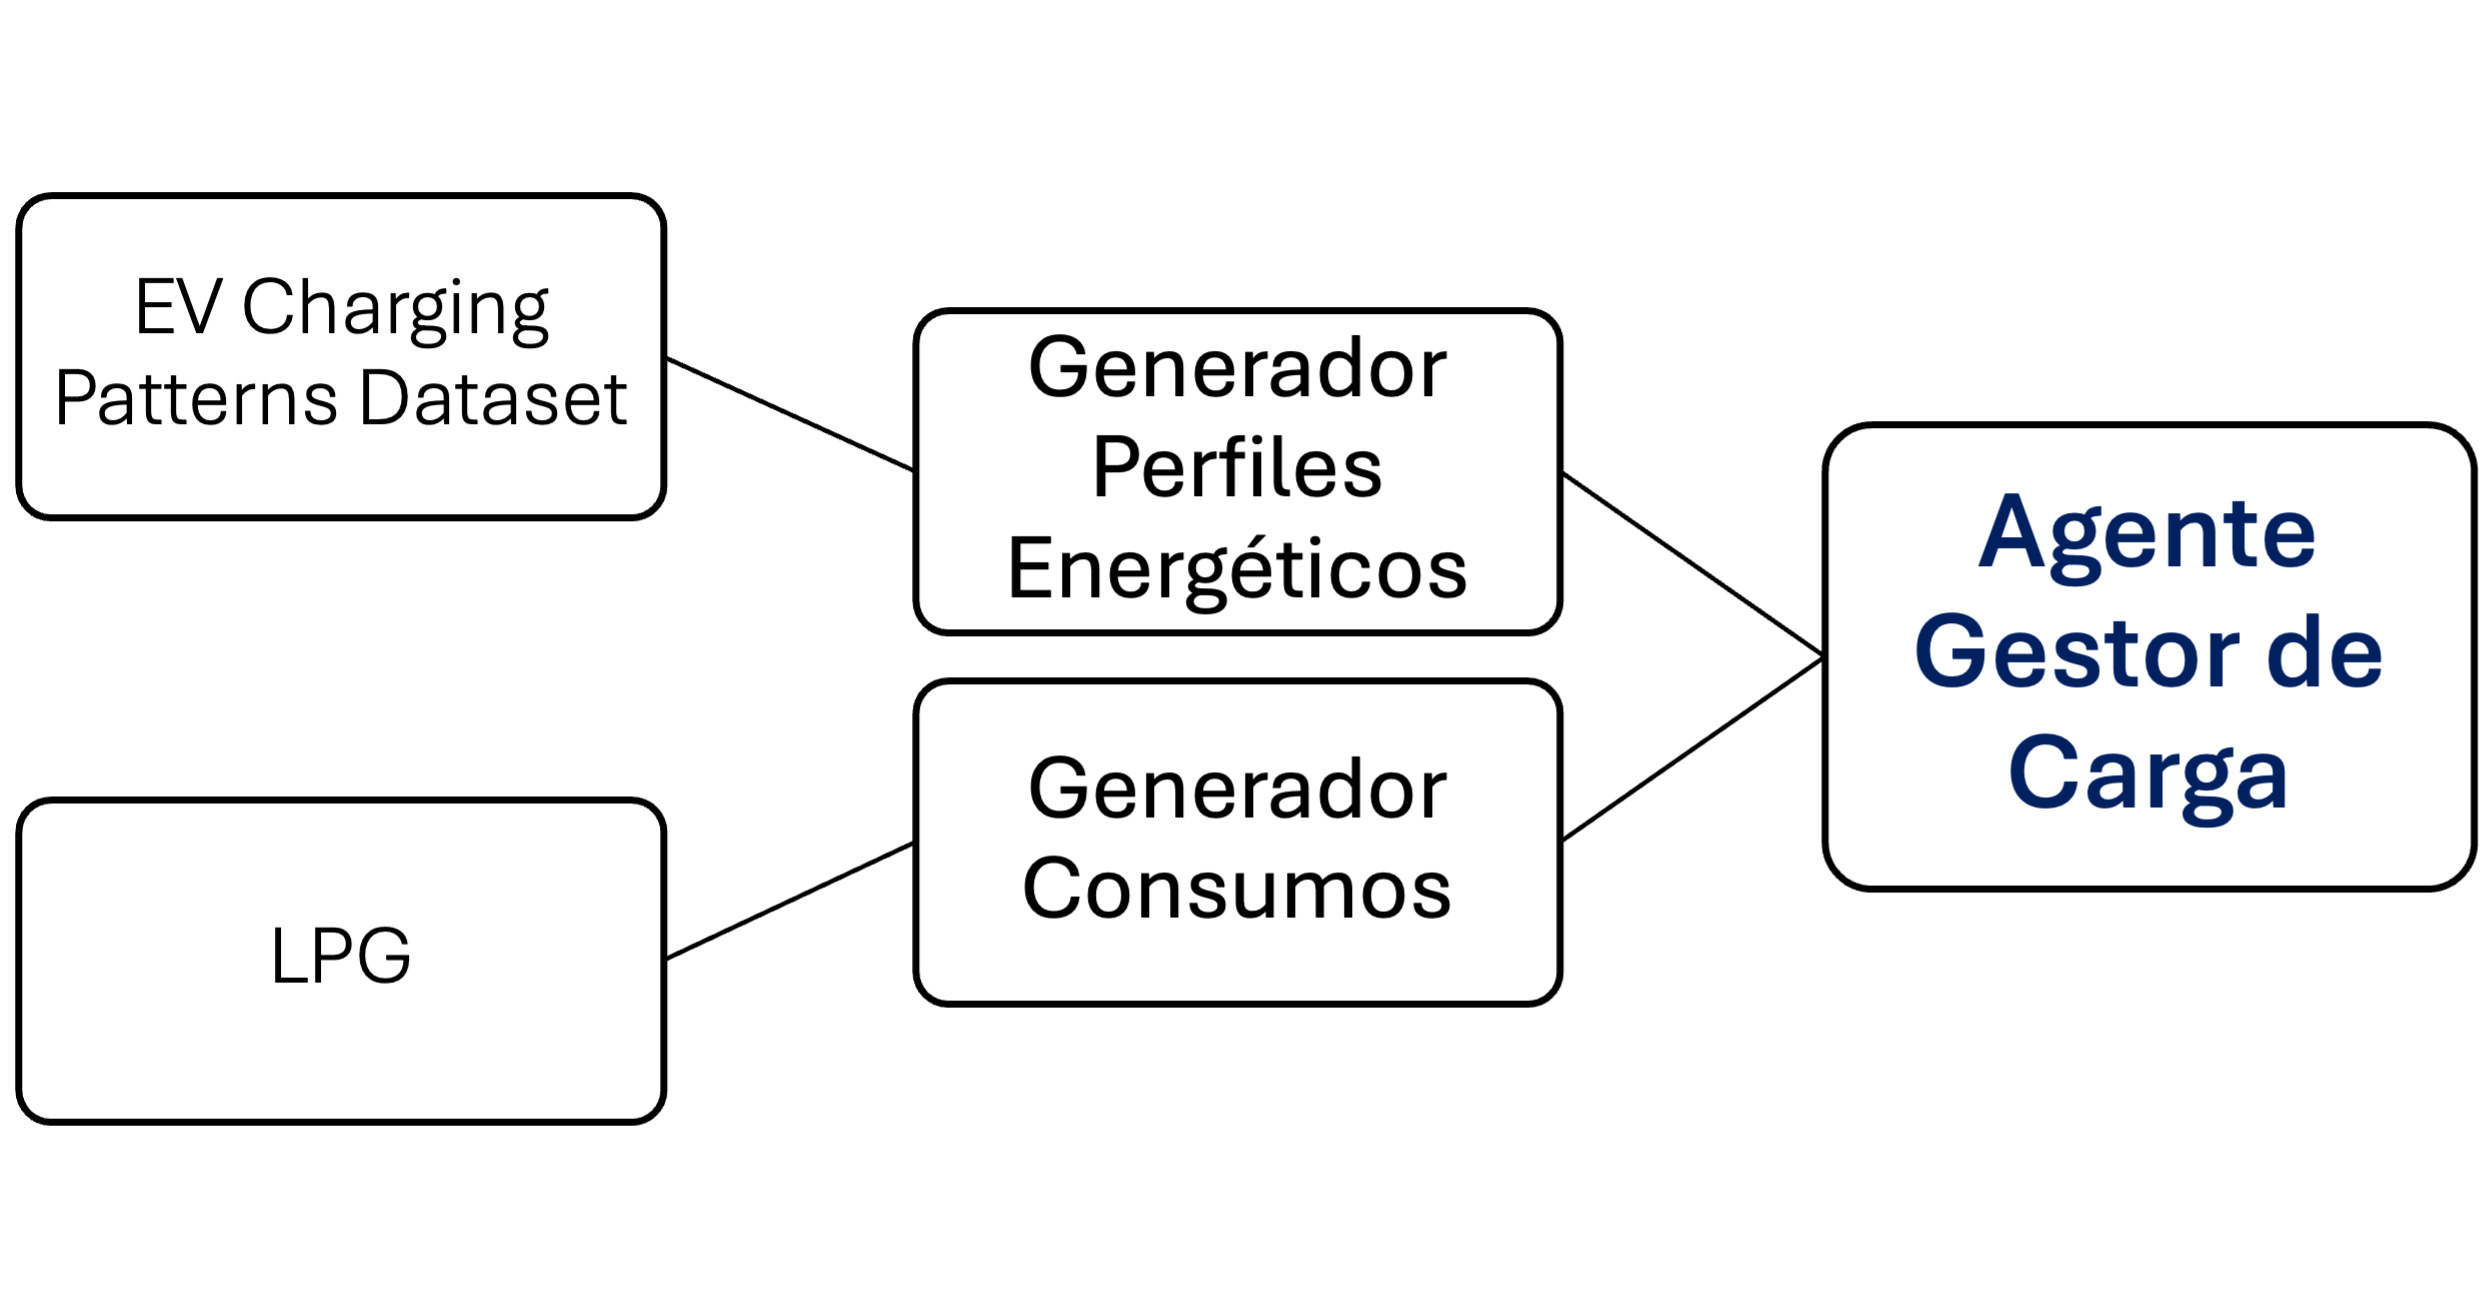
\includegraphics[width=1\textwidth]{images/metodologia.png}
    \caption{Metodología utilizada en el trabajo. Fuente: Elaboración propia.}
    \label{fig:metodologia}
\end{figure}

La metodología utilizada en este trabajo se ha diseñado para abordar de manera sistemática y 
efectiva los objetivos planteados. La Figura~\ref{fig:metodologia} ilustra las etapas clave del 
proceso, que incluyen la recopilación de datos, el análisis de la información, el desarrollo de 
modelos predictivos y la implementación de estrategias de gestión de la demanda.\\ % This is the way we should import files and partition our document.
	\cleardoublepage
	\chapter{Caso de Estudio} % This is the way we should import files and partition our document.
	\cleardoublepage
	\chapter{Resultados}
\label{chapter5}
En el capítulo anterior se ha visto cómo se desenvolían los distintos algoritmos de optimización 
intentando resolver el problema planteado en el trabajo. A lo largo de este capítulo, se va a hacer
un análisis conjunto de los resultados obtenidos por separado para cada uno de los algoritmos. Se 
hará especial hincapié en tres comparaciones fundamentales para el proyecto: coste, energía y 
rendimiento. Adicionalmente, como derivado natural de la evaluación de los costes y el consmo 
energético, se analizará también la eficiencia de cada uno de los algoritmos.

Para facilitar la comparación entre la optimización clásica y el agente DQN-LSTM, en cada sección 
se presentarán los resultados de ambos métodos en paralelo, utilizando tablas comparativas. De este 
modo, se puede observar de forma directa las diferencias y ventajas de cada enfoque para cada perfil 
analizado. Además, se puede calcular el porcentaje de diferencia (mejora o empeoramiento) de DQN-LSTM 
respecto a la optimización clásica para cada métrica relevante, lo que permite cuantificar el impacto 
de la inteligencia artificial frente a los métodos tradicionales.

\section{Comparativa de Costes}
La primera comparativa que se va a realizar es la de los costes medios diarios por perfil,
tanto para la optimización clásica como para el agente DQN-LSTM. Para ello, se muestran en la
Tabla~\ref{tab:costes_algoritmos} los costes medios diarios para cada perfil:
\begin{table}[H]
    \centering
    \resizebox{\textwidth}{!}{
    \begin{tabular}{lccc}
        \toprule
        \textbf{Perfil} & \textbf{Costes - Clásica} (EUR) & \textbf{Costes - DQN-LSTM} (EUR) & \textbf{Reducción Costes(\%)} \\
        \midrule
        retired     & 27.14 & 1.64 & 93.96 \\
        night\_owl  & 27.57 & 6.21 & 77.47 \\
        flexible    & 27.69 & 2.93 & 89.41 \\
        traveller   & 27.23 & 7.09 & 73.96 \\
        worker      & 27.35 & 5.04 & 81.57 \\
        \midrule
        \textbf{Media} & \textbf{27.40} & \textbf{4.18} & \textbf{84.74} \\
        \bottomrule
    \end{tabular}
    }
    \caption{Comparativa de costes medios diarios por perfil entre la optimización clásica y el 
    agente DQN-LSTM, junto con el porcentaje de reducción de coste.}
    \label{tab:costes_algoritmos}
\end{table}

"[pongo un gráfico en vez de la tabla??]"\\

En esta primera ronda, se puede observar fácilmente como la IA ha conseguido reducir unos datos
de coste, que ya de por sí no eran extremadamente elevados con la optimización clásica, a unas 
cifras muy reducidas. En concreto, el agente DQN-LSTM ha conseguido reducir los costes
medios diarios en un 84.74\% respecto a la optimización clásica, lo que supone una mejora
significativa en términos de eficiencia económica. Esta reducción es especialmente notable en
el perfil \textit{retired}, donde se ha alcanzado una reducción del 93.96\%. Esto se podría deber 
a que este perfil tiene un consumo energético más predecible y estable, lo que permite al
agente DQN-LSTM optimizar mejor los tiempos de carga y los costes asociados.\\

Por otro lado, el perfil \textit{night\_owl} ha mostrado una reducción del 77.47\%, lo que indica que,
aunque la optimización clásica ya era eficiente, el agente DQN-LSTM ha logrado mejorar aún más
la gestión de los tiempos de carga nocturna, aprovechando las tarifas más bajas.\\

Los perfiles \textit{flexible} y \textit{traveller} también han mostrado reducciones significativas,
con un 89.41\% y un 73.96\% respectivamente. Esto sugiere que, aunque estos perfiles pueden tener
un consumo mucho más variable, el agente DQN-LSTM ha logrado adaptarse a sus necesidades específicas,
optimizando los tiempos de carga y reduciendo los costes asociados.\\

Por último, el perfil \textit{worker} ha mostrado una reducción del 81.57\%, ligeramente por debajo
de la media, lo que indica que el agente DQN-LSTM, de nuevo, ha logrado una mejora considerable 
para este perfil también. Esto puede deberse a que los trabajadores suelen tener horarios más
predecibles, lo que permite al agente optimizar mejor los tiempos de carga y los costes asociados.\\

Cerrando este primer análisis, se puede concluir que, en este estudio, la optimización clásica queda
muy por detrás económicamente de la optimización mediante el agente DQN-LSTM, que ha conseguido 
incurrir en casi un 85\% menos de costes diarios.

\section{Comparativa de Energía}
De la misma manera que con el coste, se va a realizar una comparativa de la energía consumida por 
cada uno de los algoritmos. Para ello, se muestran en la Tabla~\ref{tab:energia_algoritmos} los 
consumos medios diarios para cada perfil, diferenciando entre la optimización clásica y el agente 
DQN-LSTM.
\begin{table}[H]
    \centering
    \resizebox{\textwidth}{!}{
    \begin{tabular}{lccc}
        \toprule
        \textbf{Perfil} & \textbf{Energía - Clásica} (kWh) & \textbf{Energía - DQN-LSTM} (kWh) & \textbf{Reducción Energía (\%)} \\
        \midrule
        retired     & 244.08 & 63.28 & 74.08 \\
        night\_owl  & 244.53 & 268.06 & -9.62 \\
        flexible    & 245.02 & 120.07 & 50.99 \\
        traveller   & 242.74 & 325.07 & -33.97 \\
        worker      & 244.08 & 209.68 & 14.12 \\
        \midrule
        \textbf{Media} & \textbf{244.09} & \textbf{197.23} & \textbf{19.21} \\
        \bottomrule
    \end{tabular}
    }
    \caption{Comparativa de energía media diaria por perfil entre la optimización clásica y el agente DQN-LSTM, junto con el porcentaje de reducción de consumo energético.}
    \label{tab:energia_algoritmos}
\end{table}

En esta comparativa se busca que el gestor, ya sea el agente DQN-LSTM o la optimización clásica,
consuma la menor cantidad de energía posible, ya que esto se traduce directamente en una reducción 
de costes en la carga. En este caso, aunque la IA ha conseguido reducir la energía consumida casi 
en un 20\% de media, no lo ha hecho de forma uniforme para todos los perfiles.\\

La mayor diferencia entre consumos se encuentra con el perfil \textit{retired}, donde la red 
neuronal consigue una reducción del 74.08\% respecto a la optimización clásica, una cifra 
tremendamente elevada. Esto puede deberse a que este perfil tiene un consumo energético mucho más 
estable y predecible, lo que permite al agente DQN-LSTM aprovechar su entorno y optimizar los tiempos
de carga para reducir el consumo energético.\\

Por otra parte, el peril night\_owl ha mostrado un aumento del 9.62\% en el consumo energético,
lo que indica que la optimización clásica ya era eficiente, y el agente DQN-LSTM no ha logrado
ni siquiera igualar ese consumo. Esto puede deberse a que este perfil tiene un consumo energético
diurno, y puede haberse visto afectado por la rareza de esta característica, ya que la mayoría del 
resto de perfiles tienen un consumo nocturno. En este caso, puede ser que la cpaacidad de memoria
de la inteligencia artificial haya sido un detrimento para su rendimiento en este perfil.\\

El perfil \textit{flexible} ha mostrado una reducción del 50.99\%, lo que muestra que el agente 
DQN-LSTM se adapta mucho mejor a la flexibilidad de carga de este perfil, contrastando con la 
rigidez de la optimización clásica. Esto sugiere que el agente ha logrado optimizar los tiempos de
carga y reducir el consumo energético, aprovechando las horas de menor demanda.\\

El perfil \textit{traveller} ha mostrado un aumento del 33.97\% en el consumo energético, lo que
indica que la optimización clásica ya era eficiente, y el agente DQN-LSTM de nuevo no ha logrado
si quiera igualar ese consumo.\\

Por último, el perfil \textit{worker} ha mostrado una reducción del 14.12\%, lo que indica que
el agente DQN-LSTM ha logrado una mejora considerable en la gestión de los tiempos de carga y el
consumo energético en el perfil más representativo, aunque no tan significativa como en el caso 
del perfil \textit{retired}. Esto puede deberse a que los trabajadores suelen tener horarios más
predecibles, lo que permite al agente optimizar mejor los tiempos de carga y reducir el consumo
energético.\\

La conclusión de esta comparativa no es del todo clara, ni positiva hacia el agente DQN-LSTM.
Aunque ha conseguido reducir el consumo energético - de media - en un 19.21\%, lo que supone una 
mejora considerable, no ha logrado igualar los resultados de la optimización clásica en todos los
perfiles. De hecho, hay un perfil en el que ha aumentado considerablemente el consumo energético 
en comparación con la gestión realizada por el algoritmo clásico. Por tanto, aunque la IA ha
conseguido una mejora significativa en la reducción de costes, no ha logrado una mejora uniforme en
el consumo energético.

\section{Comparativa de Eficiencia}
Siguiendo la misma línea que en las comparativas anteriores, se va a realizar una comparativa de la 
eficiencia de cada uno de los algoritmos. Para ello, se muestran en la Tabla~\ref{tab:eficiencia_algoritmos} 
las eficiencias medias diarias para cada perfil, diferenciando entre la optimización clásica y el 
agente DQN-LSTM. La eficiencia se calcula como el cociente entre la energía consumida y el coste, 
es decir, \( \text{Eficiencia} = \frac{\text{Energía}}{\text{Coste}} \).
\begin{table}[H]
    \centering
    \resizebox{\textwidth}{!}{
    \begin{tabular}{lccc}
        \toprule
        \textbf{Perfil} & \textbf{Eficiencia - Clásica} (kWh/EUR) & \textbf{Eficiencia - DQN-LSTM} (kWh/EUR) & \textbf{Mejora Eficiencia(\%)} \\
        \midrule
        retired     & 8.99  & 37.14 & 313.16 \\
        night\_owl  & 8.87  & 43.07 & 385.77 \\
        flexible    & 8.85  & 40.33 & 355.99 \\
        traveller   & 8.92  & 45.93 & 415.13 \\
        worker      & 8.92  & 41.63 & 366.77 \\
        \midrule
        \textbf{Media} & \textbf{8.91} & \textbf{41.62} & \textbf{367.18} \\
        \bottomrule
    \end{tabular}
    }
    \caption{Comparativa de la eficiencia diaria (kWh/EUR) por perfil entre la optimización clásica y el agente DQN-LSTM, junto con el porcentaje de mejora en eficiencia.}
    \label{tab:eficiencia_algoritmos}
\end{table}

La eficiencia es una métrica que combina el coste y el consumo energético, y dado la disparidad en 
los resultados de las dos comparativas anteriores, se espera que la eficiencia sea una métrica más
representativa del rendimiento de cada uno de los algoritmos. Naturalmente, al representar esta
medida, esencialmente, la cantidad de kWh que usados por cada euro invertido, cuanto mayor sea el
valor, mejor.\\

En este caso sí, la red neuronal ha pasado por encima de la optimización clásica en todos los perfiles.
Tanto es así, que no merece la pena el análisis de cada perfil individualmente, ya que la mejora es
de tal magnitud que se puede considerar como una gran mejora generalizada. En concreto, el agente 
DQN-LSTM ha conseguido una mejora de la eficiencia del 367.18\% respecto a la optimización clásica,
una diferencia abismal que demuestra la capacidad de la IA para optimizar los tiempos de carga y reducir
los costes asociados.\\

Si bien es cierto que esta métrica deriva de las dos anteriores, y por tanto, no es una métrica
independiente. Por ello, podría estar sesgada por los resultados de las comparativas de coste y 
energía. Sin embargo, la magnitud de la mejora es tal, que puede considerarse una mejora 
significativa y representativa del rendimiento del agente DQN-LSTM frente a la optimización 
clásica.

\section{Comparativa de Rendimiento}
Finalmente, se va a realizar una comparativa del rendimiento de cada uno de los algoritmos.
Para ello, se muestran en la Tabla~\ref{tab:rendimiento_algoritmos} los rendimientos medios para 
ambos algoritmos. El rendimiento en este caso se va a basar en el tiempo de ejecución y de decisión/
inferencia de cada uno de los algoritmos. Se ha medido el tiempo medio de ejecución/entrenamiento de
cada uno de los algoritmos, así como el tiempo medio de decisión/inferencia.\\

En general, la optimización clásica suele requerir menos tiempo de cálculo para problemas 
individuales, pero no es escalable ni adaptable a cambios dinámicos. Por otro lado, el agente DQN-
LSTM requiere un tiempo de entrenamiento inicial mayor, pero una vez entrenado, la inferencia es 
extremadamente rápida y permite adaptarse a nuevas situaciones en tiempo real.

\begin{table}[H]
    \centering
    \begin{tabular}{lccc}
        \toprule
        \textbf{Perfil} & \textbf{Tiempo total (min)} & \textbf{Tiempo de Solución (ms)} & \textbf{Método} \\
        \midrule
        worker      & 0.13\footnotemark[1] & 9.50\footnotemark[2] & Clásica \\
        flexible    & 0.13\footnotemark[1] & 9.50\footnotemark[2] & Clásica \\
        retired     & 0.13\footnotemark[1] & 9.50\footnotemark[2] & Clásica \\
        traveller   & 0.13\footnotemark[1] & 9.50\footnotemark[2] & Clásica \\
        night\_owl  & 0.13\footnotemark[1] & 9.50\footnotemark[2] & Clásica \\
        \midrule
        worker      & 3.98 & 0.174 & DQN-LSTM \\
        flexible    & 4.39 & 0.294 & DQN-LSTM \\
        retired     & 4.29 & 0.301 & DQN-LSTM \\
        traveller   & 4.45 & 0.309 & DQN-LSTM \\
        night\_owl  & 4.37 & 0.306 & DQN-LSTM \\
        \bottomrule
    \end{tabular}
    \caption{Comparativa de tiempos de entrenamiento/optimización total y de inferencia/decisión 
    por perfil y método. Para la optimización clásica, el tiempo total corresponde al tiempo total 
    de optimización (8.05 s $\approx$ 0.13 min) y el tiempo de inferencia al tiempo resolviendo 
    modelos individuales (0.57 s / 60 $\approx$ 9.50 ms por perfil).}
\end{table}

\footnotetext[1]{Tiempo total de optimización clásica para todos los perfiles.}
\footnotetext[2]{Tiempo de inferencia de la optimización clásica para cada perfil.}

El análisis de rendimiento computacional, es decir, cuanto tiempo requiere cada programa para 
resolver el problema para cada uno de los perfiles, es un aspecto fundamental del trabajo. De cara 
a la implementación de un sistema real, es necesario que el tiempo de respuesta y las demandas 
computacionales sean lo más bajas posibles, para que el sistema pueda adaptarse a las
necesidades de los usuarios en tiempo real, sin pérdidas en la calidad del servicio ni requisitos 
de hardware excesivos.\\

Por la naturaleza de los algoritmos, es necesario dividir la comparación en dos partes: el tiempo
que requiere cada algooritmo para optimizar el problema como tal, con todas las iteraciones y
entrenamientos necesarios; y el tiempo que requiere cada algoritmo para inferir o llegra a una 
solución para una instancia concreta del problema.\\

En la primera de las comparativas, es evidente que la red neuronal es mucho más lenta y 
computacionalmente intensiva que la optimización clásica. Esto, además de esperado, es lógico, ya 
que la optimizción clásica es un algoritmo iterativo que resuelve el problema de forma directa. Sin
memoria, sin entrenamiento ni aprendizaje, simplemente resuelve el problema de forma
determinista.\\

En cambio, el agente DQN-LSTM requiere un tiempo de entrenamiento inicial mucho mayor, por las 
razones opuestas al algoritmo clásico. La red neuronal sí debe aprender de los datos,
requiere un entrenamiento previo y, por tanto, un tiempo de optimización mucho mayor. Además, con
la dificultad añadida de la incorporación de unas capas de LSTM, cuya función es esencial para el 
más que adecuado funcionamiento de la red, pero incrementa el tiempo de entrenamiento y los recursos
computacionales necesarios.\\

Sin embargo, una vez entrenada, la red neuronal es mucho más capaz que la optimización clásica
para resolver problemas individuales. En este caso, el mejor tiempo de inferencia del agente DQN-LSTM
es incluso menor que el 2,5\% del tiempo de inferencia de la optimización clásica.
Esto se debe a que, una vez entrenada, la red neuronal puede inferir soluciones de forma casi
instantánea, ya que no requiere volver a resolver el problema desde cero, sino que utiliza el
conocimiento adquirido durante el entrenamiento para tomar decisiones rápidas y eficientes.\\

Por tanto, aunque la optimización clásica es más rápida en términos de tiempo total de optimización,
el agente DQN-LSTM es mucho más eficiente en términos de tiempo de inferencia, lo que lo hace
más adecuado para aplicaciones en tiempo real donde se requiere una respuesta rápida y adaptativa.\\ % This is the way we should import files and partition our document.
	\cleardoublepage
	\chapter{Conclusiones y Trabajo Futuro}
\section{Conclusiones}
En este trabajo se ha presentado un sistema de predicción y gestión de la demanda energética para 
la carga de vehículos eléctricos, utilizando un enfoque de modelado híbrido que combina técnicas 
de aprendizaje automático y aprendizaje por refuerzo con memoria, basado en IA generativa.\\

Tanto el optimizador clásico como el sistema de IA generativa han resultado eficaces para gestionar 
la carga de vehículos eléctricos bajo las restricciones planteadas. El enfoque clásico, mediante 
programación lineal, ha ofrecido soluciones óptimas en coste y eficiencia, respetando tanto los 
límites técnicos como las preferencias del usuario. Por su parte, la IA generativa ha destacado por 
su capacidad de adaptación ante escenarios variables, logrando minimizar costes y aprovechar al 
máximo la energía disponible, siempre dentro de los requisitos establecidos.\\

También se ha logrado generar perfiles sintéticos de demanda y disponibilidad de energía con la 
ayuda de técnicas de IA Generativa, lo que ha permitido simular escenarios realistas para la carga 
de vehículos eléctricos.

Finalmente, tras un análisis comparativo de los resultados obtenidos por ambos enfoques, se ha
concluido que, aunque el optimizador clásico garantiza soluciones óptimas bajo restricciones
específicas, el sistema de IA generativa ofrece una mayor flexibilidad y adaptabilidad a cambios
en las condiciones de carga y disponibilidad de energía. Esto lo convierte en una herramienta valiosa
para la planificación y operación de sistemas energéticos cada vez más complejos, especialmente en
el contexto de la movilidad eléctrica y la integración de energías renovables.\\

\section{Próximos Pasos}
Aunque el sistema desarrollado ha demostrado ser eficaz y cumple con los objetivos planteados,
existen varias áreas de mejora y expansión que podrían explorarse en el futuro:
\begin{itemize}
    \item \textbf{Introducción de algoritmos de clustering:} Incorporar técnicas como 
    \textit{k-means} \cite{lloyd1982kmeans} o \textit{k-nearest neighbors} \cite{altman1992knn} para 
    identificar y clasificar perfiles de demanda y patrones de carga, permitiendo una gestión 
    más personalizada y eficiente de los recursos energéticos.
    \item \textbf{Mejora de la política de control mediante métodos Actor-Critic:} Implementar 
    enfoques avanzados de aprendizaje por refuerzo, como métodos Actor-Critic o políticas de 
    gradiente, que permitan asignar recompensas suaves (\textit{soft rewards}) en función de la 
    dirección y calidad de las acciones tomadas por el sistema, facilitando un aprendizaje más fino 
    y adaptativo.
    \item \textbf{Capacidades predictivas avanzadas:} Integrar modelos de predicción para anticipar 
    la demanda energética y la disponibilidad de recursos, mejorando la planificación y la toma de 
    decisiones en tiempo real.
    \item \textbf{Ampliación de la memoria y el \textit{replay buffer}:} Aumentar la capacidad de 
    memoria del sistema, permitiendo el acceso a experiencias pasadas relevantes, como datos de 
    fechas o situaciones similares de años anteriores, para enriquecer el aprendizaje y la toma de 
    decisiones.
    \item \textbf{Integración de energías renovables en el consumo no gestionable:} Considerar la 
    aportación de fuentes renovables en la parte de la demanda no gestionable, incrementando la 
    sostenibilidad y la eficiencia global del sistema.
\end{itemize} % This is the way we should import files and partition our document.
	\cleardoublepage
	%% Include more chapters and or documents.
	
	\appendix
	
	%% Include appendixes
	
	\cleardoublepage
	
	\printbibliography[heading=bibintoc] % We print the entire bibliography of the document. The author recommends that, if the document contains tremendous amounts of references, that they should be written at the end of each chapter. Refer to https://www.overleaf.com/learn/latex/Bibliography_management_in_LaTeX for more information.
	
	\backmatter
	
\end{document}
